%----------------------------------------------------------------------------
\section{Behaviour Models}\label{sec:behaviour_models}
%----------------------------------------------------------------------------

\subsection{Finite State Machine}

Finite state machines (FSMs) are widely used formalisms to model computation. They can be in exactly one of a finite number of \emph{states} at any given time. FSM can change from one state to another in response to some \emph{inputs} (usually called signals); which change is called a \emph{transition} (see \autoref{fig:fsm} for an example finite state machine).

\begin{figure}[!ht]
	\centering
	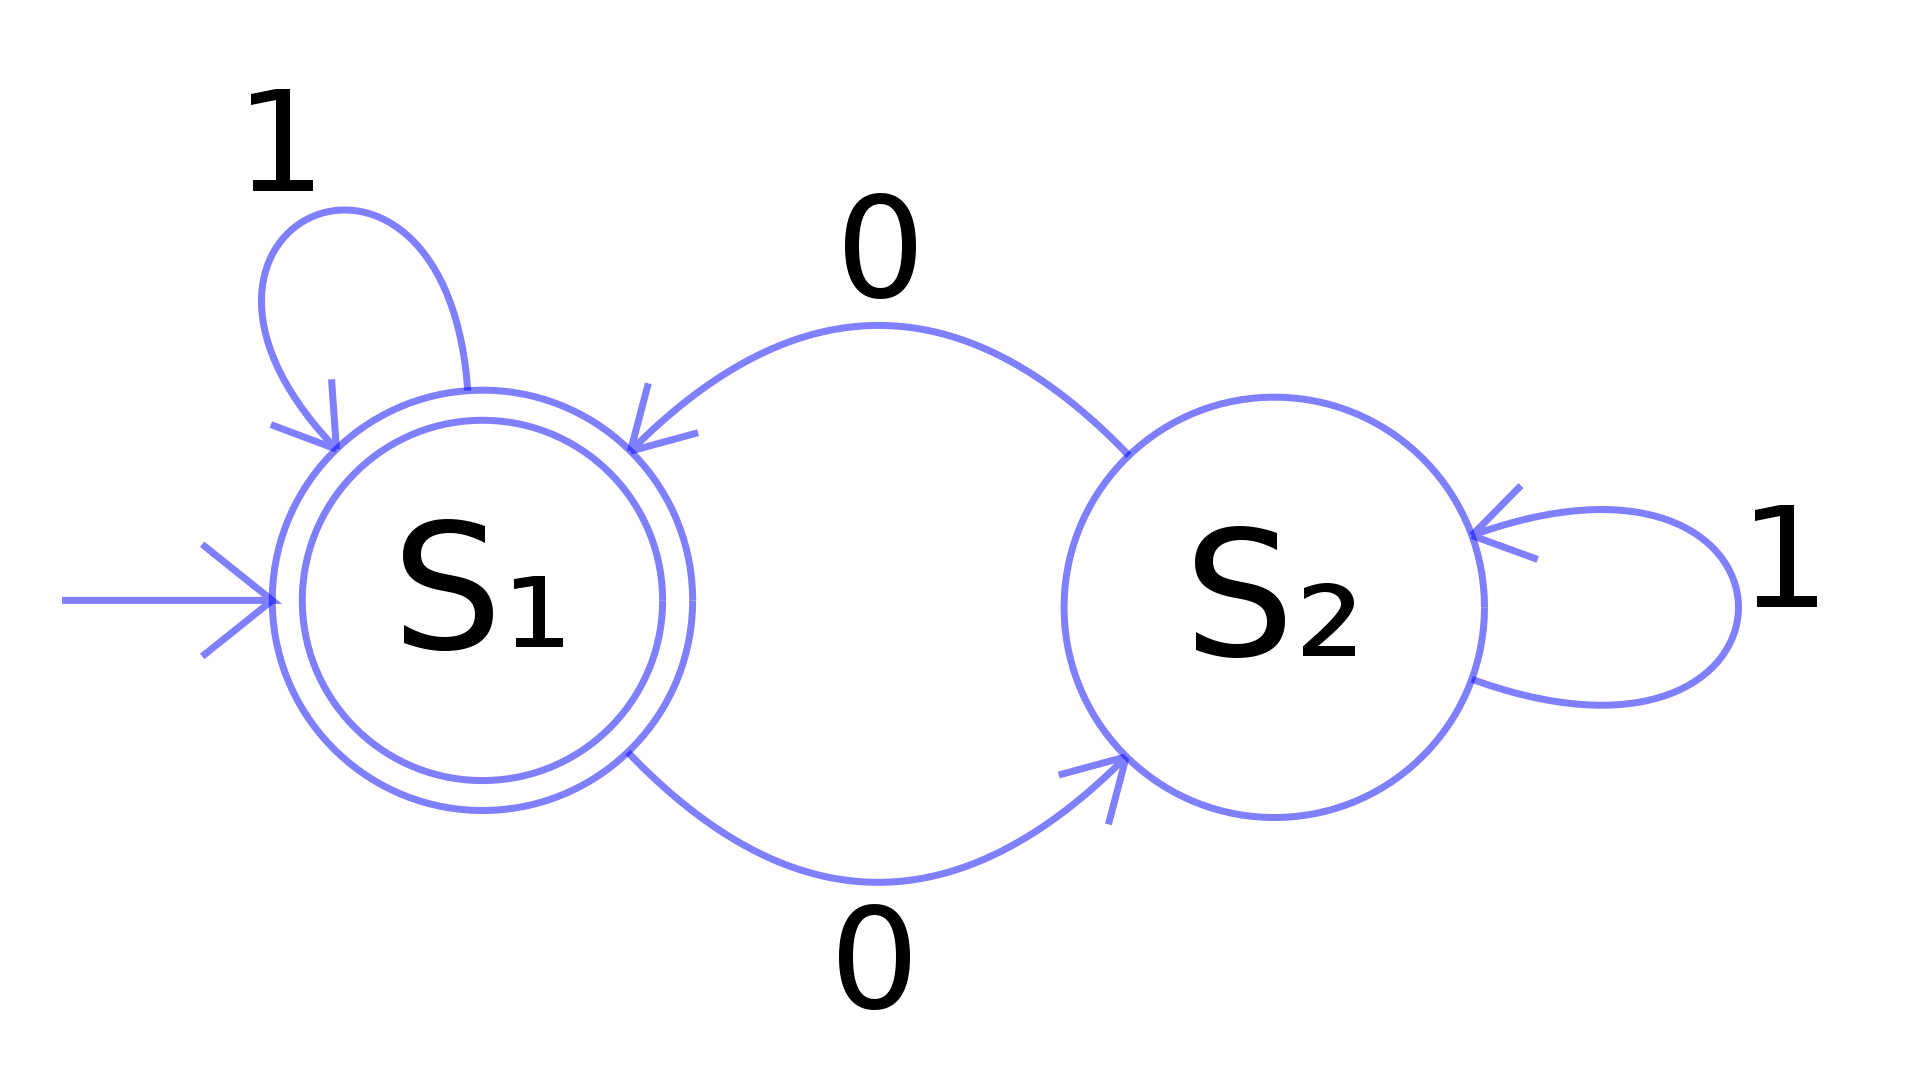
\includegraphics[width=67mm, keepaspectratio]{figures/fsm.png}\hspace{1cm}
	\caption{An example deterministic finite state machine, which checks a given binary numbers \emph{evenness}.}
	\label{fig:fsm}
\end{figure}

The formal definition of \emph{deterministic} finite state machines is as follows.

\begin{definition}[Deterministic finite state machine]
	
	A DFSM is a tuple \( SM = (\Sigma, S, s_0, \delta, F) \)
	
	\begin{itemize}
		\item \(\Sigma\) is the set input \emph{alphabet} (a finite non-empty set of symbols);
		\item \(S\) is a finite non-empty set of states;
		\item \(s_0 \in S\) is an initial state;
		\item \(\delta : S \times \Sigma \rightarrow S \) is the state-transition function;
		\item \(F \subseteq S\) is the set of final states
	\end{itemize}
\end{definition}

The current state of a DFSM is \(s \in S\). A transition from state to state is performed, given the last input letter \(l\), if and only if \( s' = \delta(s, l) \in S \). In which case the current state will become \(s'\) (this work assumes, that if the given \(\delta(s, l)\) is not defined, then the state machine remains in it's current state)).

\subsection{Petri Net}

\begin{figure}[!ht]
	\centering
	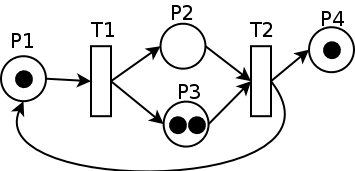
\includegraphics[width=67mm, keepaspectratio]{figures/petri_net.png}\hspace{1cm}
	\caption{An example Petri net with 2 transitions and 4 places.}
	\label{fig:petri_net}
\end{figure}

Petri nets are a widely used formalism to model concurrent, asynchronous systems \cite{24143}. The formal definition of a Petri net (including inhibitor arcs) is as follows (see \autoref{fig:petri_net} for an illustration of the notations).

\begin{definition}[Petri net]
	
	A Petri net is a tuple \( PN = (P, T, W, M_0) \)
	
	\begin{itemize}
		\item \(P\) is the set of \emph{places} (defining state variables);
		\item \(T\) is the set of \emph{transitions} (defining behaviour), such that \( P \bigcap T = \emptyset \);
		\item \(W \subseteq W^+ \bigcup W^- \) is a set of two types of arcs, where \(  W^+ : T \times P \rightarrow \mathbb{N}\) and \( W^- : P \times T \rightarrow \mathbb{N} \) are the set of input arcs and output arcs, respectively (\( \mathbb{N} \) is the set of all natural numbers);
		\item \(M_0 : P \rightarrow \mathbb{N} \) is the \emph{initial marking}, i.e., the number of \emph{tokens} on each place.
	\end{itemize}
\end{definition}

The state of a Petri net is defined by the current marking \( M : P \rightarrow \mathbb{N} \). The behaviour of the systems is described as follows. A transition \( t \) is enabled if \( \forall p \in P : M(p) \in W(p, t) \). Any enabled transition \(t\) may fire non-deterministically, creating the new marking \( M' \) of the Petri as follows: \( \forall p \in P : M'(p) = M(p) - W^-(p, t) + W^+(t, p) \).

In words: W describes the \emph{weight} of each flow from a transition to a place, or from a place to a transition. Firing a transition \(t\) in a marking \(M\) consumes \(W^-(p_i, t)\) tokens from each of its input places \(p_i\), and produces \(W(t, p_o)\) tokens in each of its output places \(p_o\). One such transition \(t\) is \emph{enabled} (it may \emph{fire}) in \(M\) if there are enough tokens in its input places for the consumptions to be possible, i.e., if and only if \( \forall p : M(p) \ge W(s, t)\).

\subsection{Differences}

In real world applications, both behaviour models are useful, but for different use-cases. State machines provide a way of specifying what our system \emph{react} with, when a given \emph{environmental} event happens. This could be a user interaction (e.g., a keystroke) or a new temperature reading.

On the other hand, petri nets provide a way of modeling distributed systems with many interconnecting components, all running on their own accords. They have dependencies on each other (one calculates a value the other needs), or have a limited resource (a factory only has one worker).
